\documentclass[aspectratio=169,11pt]{beamer}
% =====================================================================
%  pds-beamer.tex — Estilo común de las transparencias.
%
%  Uso (desde teoría/Tx/transparencias/):
%     \documentclass[aspectratio=169,11pt]{beamer}
%     % =====================================================================
%  pds-beamer.tex — Estilo común de las transparencias.
%
%  Uso (desde teoría/Tx/transparencias/):
%     \documentclass[aspectratio=169,11pt]{beamer}
%     % =====================================================================
%  pds-beamer.tex — Estilo común de las transparencias.
%
%  Uso (desde teoría/Tx/transparencias/):
%     \documentclass[aspectratio=169,11pt]{beamer}
%     \input{../../comun/pds-beamer}
%     \title{...}  \subtitle{Tema x · ...}
%     \begin{document}
%       \portada
%       ...
%     \end{document}
%  Compilar con:  latexmk -xelatex  (o «make» desde teoría/)
% =====================================================================

\usetheme{Boadilla}
\usecolortheme{orchid}
\usefonttheme{professionalfonts}
\setbeamercovered{transparent}
\setbeamersize{text margin left=0.8cm, text margin right=0.8cm}
\setbeamertemplate{navigation symbols}{}
\setbeamertemplate{itemize item}[square]
\setbeamertemplate{itemize subitem}[circle]
\setbeamertemplate{itemize subsubitem}[triangle]
\setbeamertemplate{enumerate item}[square]
\setbeamertemplate{enumerate subitem}[circle]
\setbeamertemplate{caption}{\raggedright\insertcaption\par}

\input{../../comun/pds-comun.tex}

% Tipografía: Fira Sans + Fira Math (legibles en proyector)
\usepackage{fontspec}
\usepackage{unicode-math}
% Se cargan por nombre de fichero para que funcionen con cualquier
% instalación de TeX Live (o MiKTeX) sin instalar fuentes en el sistema.
\setmainfont{FiraSans}[Extension=.otf, UprightFont=*-Regular, BoldFont=*-SemiBold,
  ItalicFont=*-Italic, BoldItalicFont=*-SemiBoldItalic]
\setsansfont{FiraSans}[Extension=.otf, UprightFont=*-Regular, BoldFont=*-SemiBold,
  ItalicFont=*-Italic, BoldItalicFont=*-SemiBoldItalic]
\setmonofont{FiraMono}[Extension=.otf, UprightFont=*-Regular, BoldFont=*-Medium, AutoFakeSlant=0.15, Scale=0.92]
\setmathfont{FiraMath-Regular.otf}
\setmathfont{latinmodern-math.otf}[range={"229B,"22EE,"22F1}]

% Colores del tema ajustados a la paleta común (más contraste)
\setbeamercolor{structure}{fg=pdsazul}
\setbeamercolor{alerted text}{fg=pdsrojo}
\setbeamercolor{example text}{fg=pdsverde}
\setbeamercolor{block title}{bg=pdsazul, fg=white}
\setbeamercolor{block body}{bg=pdsfondo}
\setbeamercolor{block title alerted}{bg=pdsrojo, fg=white}
\setbeamercolor{block body alerted}{bg=pdsrojo!6}
\setbeamercolor{block title example}{bg=pdsverde, fg=white}
\setbeamercolor{block body example}{bg=pdsverde!6}
\setbeamercolor{frametitle}{fg=pdsazul, bg=white}
\setbeamerfont{frametitle}{size=\large, series=\bfseries}
\setbeamerfont{block title}{size=\normalsize, series=\bfseries}
\setbeamertemplate{blocks}[rounded][shadow=false]

% Logo en la esquina superior derecha de cada transparencia
\pgfdeclareimage[height=0.8cm]{logo}{../../comun/ucm.png}
\addtobeamertemplate{frametitle}{}{%
  \begin{tikzpicture}[remember picture, overlay]
    \node[anchor=north east, inner sep=0pt] at ([xshift=-0.25cm, yshift=-0.2cm]current page.north east) {\pgfuseimage{logo}};
  \end{tikzpicture}}

% Datos de portada
\author[\autorescorto]{\autores}
\institute[UCM]{\footnotesize\departamento\\\universidad}
\date[\curso]{\footnotesize\grado\\\curso}

\newcommand{\portada}{%
  \begin{frame}[plain]
    \begin{center}
      
\includegraphics[height=1.9cm]{../../comun/ucm.png}
    \end{center}
    \vspace{-0.4cm}
    \titlepage
  \end{frame}}

% Índice al empezar cada sección
\AtBeginSection[]{%
  \begin{frame}{Contenido}
    \tableofcontents[currentsection, hideothersubsections]
  \end{frame}}

\renewcommand{\pdscodesize}{\scriptsize}

% Utilidades
% \herramienta{T1-convolucion-continua}: enlace a la página publicada de
% herramientas/html (se abre en el navegador, sin instalar nada).
% \herramientaservidor{server/....py}: app que necesita Python (bokeh serve).
\newcommand{\urlherramientas}{https://ucm-237.github.io/PdS/}
\newcommand{\herramienta}[1]{%
  \par\vfill\hfill{\scriptsize\color{pdsgris}\faIcon\ \href{\urlherramientas#1.html}{Herramienta interactiva: \texttt{#1}}}}
\newcommand{\herramientaservidor}[1]{%
  \par\vfill\hfill{\scriptsize\color{pdsgris}\faIcon\ Herramienta interactiva (con Python): \texttt{herramientas/#1}}}
\newcommand{\faIcon}{\textbf{▶}}
\newcommand{\gris}[1]{{\color{pdsgris}#1}}
\newcommand{\nota}[1]{\par\vspace{2pt}{\footnotesize\color{pdsgris}\textit{#1}}\par}
% Nota sobre una errata de versiones anteriores (solo con \ERRATAS)
\newcommand{\errata}[1]{\iferratas\nota{Errata de versiones anteriores: #1}\fi}
\newcommand{\apuntes}[1]{\nota{Más detalle en los apuntes, #1.}}

% Bloques con nombre en castellano
\newenvironment{definicion}[1][Definición]{\begin{block}{#1}}{\end{block}}
\newenvironment{importante}[1][Importante]{\begin{alertblock}{#1}}{\end{alertblock}}
\newenvironment{ejemplo}[1][Ejemplo]{\begin{exampleblock}{#1}}{\end{exampleblock}}

%     \title{...}  \subtitle{Tema x · ...}
%     \begin{document}
%       \portada
%       ...
%     \end{document}
%  Compilar con:  latexmk -xelatex  (o «make» desde teoría/)
% =====================================================================

\usetheme{Boadilla}
\usecolortheme{orchid}
\usefonttheme{professionalfonts}
\setbeamercovered{transparent}
\setbeamersize{text margin left=0.8cm, text margin right=0.8cm}
\setbeamertemplate{navigation symbols}{}
\setbeamertemplate{itemize item}[square]
\setbeamertemplate{itemize subitem}[circle]
\setbeamertemplate{itemize subsubitem}[triangle]
\setbeamertemplate{enumerate item}[square]
\setbeamertemplate{enumerate subitem}[circle]
\setbeamertemplate{caption}{\raggedright\insertcaption\par}

% =====================================================================
%  pds-comun.tex — Paquetes, colores y estilos de código comunes a
%  transparencias, apuntes y hojas de ejercicios. Compilar con XeLaTeX.
%  No cargar directamente: lo cargan pds-beamer.tex y pds-apuntes.tex.
% =====================================================================

\usepackage{polyglossia}
\setmainlanguage{spanish}
\usepackage{mathtools}
\usepackage{graphicx}
\usepackage{booktabs}
\usepackage{multirow}
\usepackage{array}
\usepackage{xcolor}
\usepackage{tikz}
\usetikzlibrary{positioning,arrows.meta,calc,shapes.geometric,decorations.pathreplacing}
\usepackage{listings}
\usepackage{siunitx}
\sisetup{output-decimal-marker={,}, group-separator={\,}, per-mode=symbol}

% Notas de erratas de versiones anteriores: no se imprimen salvo que se
% defina \ERRATAS antes de cargar el estilo (make ERRATAS=1)
\newif\iferratas
\ifdefined\ERRATAS \erratastrue \fi

% Ruta común (logo y figuras compartidas)
\providecommand{\rutacomun}{../../comun/}
\input{\rutacomun datos.tex}

% ---------------------------------------------------------------------
%  Paleta (la misma que usan las figuras generadas con Python,
%  ver comun/pds_estilo.py)
% ---------------------------------------------------------------------
\definecolor{pdsazul}{HTML}{2B3A8C}
\definecolor{pdsrojo}{HTML}{C0392B}
\definecolor{pdsverde}{HTML}{1E7B4F}
\definecolor{pdsnaranja}{HTML}{D9822B}
\definecolor{pdsgris}{HTML}{5A5A66}
\definecolor{pdsfondo}{HTML}{F3F4FA}
\definecolor{pdscodigo}{HTML}{F7F7F2}

% ---------------------------------------------------------------------
%  Diagramas de bloques (TikZ)
% ---------------------------------------------------------------------
\tikzset{
  bloque/.style={rectangle, rounded corners=2pt, draw=pdsazul!80, fill=pdsfondo,
                 very thick, minimum height=8mm, minimum width=14mm, align=center},
  sumador/.style={circle, draw=pdsazul!80, fill=pdsfondo, thick, inner sep=1.5pt},
  flecha/.style={-{Stealth[length=2.2mm]}, thick, pdsgris},
}

% ---------------------------------------------------------------------
%  Código: Python y Matlab en paralelo
% ---------------------------------------------------------------------
\newcommand{\pdscodesize}{\footnotesize}
\lstdefinestyle{pds}{
  basicstyle=\ttfamily\pdscodesize,
  keywordstyle=\color{pdsazul}\bfseries,
  commentstyle=\color{pdsverde}\itshape,
  stringstyle=\color{pdsrojo},
  numbers=none,
  backgroundcolor=\color{pdscodigo},
  frame=single, rulecolor=\color{pdsgris!40}, framerule=0.4pt,
  xleftmargin=2pt, xrightmargin=2pt, aboveskip=2pt, belowskip=2pt,
  columns=fullflexible, keepspaces=true,
  showstringspaces=false, breaklines=true, tabsize=4,
  upquote=true,
  % Con XeLaTeX, listings desordena los caracteres no ASCII junto a
  % dígitos («2π» sale «π2»): se sustituyen por su versión matemática.
  literate={π}{{$\pi$}}1 {δ}{{$\delta$}}1 {ω}{{$\omega$}}1 {Ω}{{$\Omega$}}1
           {≈}{{$\approx$}}1 {µ}{{$\mu$}}1 {·}{{$\cdot$}}1 {α}{{$\alpha$}}1
           {á}{{á}}1 {é}{{é}}1 {í}{{í}}1 {ó}{{ó}}1 {ú}{{ú}}1 {ñ}{{ñ}}1 {¿}{{¿}}1,
}
\lstdefinestyle{python}{style=pds, language=Python,
  morekeywords={as,True,False,None}}
\lstdefinestyle{matlab}{style=pds, language=Matlab,
  morekeywords={function,end,true,false}}

% \codigo{<ruta sin extensión>} muestra el mismo ejemplo en Python
% y en Matlab, uno al lado del otro. Los ficheros viven en
% ../codigo/python/<nombre>.py y ../codigo/matlab/<nombre>.m y se
% ejecutan en las pruebas (make prueba-codigo).
\newcommand{\rutacodigo}{../codigo/}
\newcommand{\codigoetiqueta}[1]{{\sffamily\scriptsize\bfseries\color{pdsgris}#1}}
\newcommand{\codigo}[2][]{%
  \par\noindent
  \begin{minipage}[t]{0.495\linewidth}
    \codigoetiqueta{Python}\par\vspace{1pt}
    \lstinputlisting[style=python,#1]{\rutacodigo python/#2.py}
  \end{minipage}\hfill
  \begin{minipage}[t]{0.495\linewidth}
    \codigoetiqueta{Matlab}\par\vspace{1pt}
    \lstinputlisting[style=matlab,#1]{\rutacodigo matlab/#2.m}
  \end{minipage}\par}

\input{\rutacomun notacion.tex}


% Tipografía: Fira Sans + Fira Math (legibles en proyector)
\usepackage{fontspec}
\usepackage{unicode-math}
% Se cargan por nombre de fichero para que funcionen con cualquier
% instalación de TeX Live (o MiKTeX) sin instalar fuentes en el sistema.
\setmainfont{FiraSans}[Extension=.otf, UprightFont=*-Regular, BoldFont=*-SemiBold,
  ItalicFont=*-Italic, BoldItalicFont=*-SemiBoldItalic]
\setsansfont{FiraSans}[Extension=.otf, UprightFont=*-Regular, BoldFont=*-SemiBold,
  ItalicFont=*-Italic, BoldItalicFont=*-SemiBoldItalic]
\setmonofont{FiraMono}[Extension=.otf, UprightFont=*-Regular, BoldFont=*-Medium, AutoFakeSlant=0.15, Scale=0.92]
\setmathfont{FiraMath-Regular.otf}
\setmathfont{latinmodern-math.otf}[range={"229B,"22EE,"22F1}]

% Colores del tema ajustados a la paleta común (más contraste)
\setbeamercolor{structure}{fg=pdsazul}
\setbeamercolor{alerted text}{fg=pdsrojo}
\setbeamercolor{example text}{fg=pdsverde}
\setbeamercolor{block title}{bg=pdsazul, fg=white}
\setbeamercolor{block body}{bg=pdsfondo}
\setbeamercolor{block title alerted}{bg=pdsrojo, fg=white}
\setbeamercolor{block body alerted}{bg=pdsrojo!6}
\setbeamercolor{block title example}{bg=pdsverde, fg=white}
\setbeamercolor{block body example}{bg=pdsverde!6}
\setbeamercolor{frametitle}{fg=pdsazul, bg=white}
\setbeamerfont{frametitle}{size=\large, series=\bfseries}
\setbeamerfont{block title}{size=\normalsize, series=\bfseries}
\setbeamertemplate{blocks}[rounded][shadow=false]

% Logo en la esquina superior derecha de cada transparencia
\pgfdeclareimage[height=0.8cm]{logo}{../../comun/ucm.png}
\addtobeamertemplate{frametitle}{}{%
  \begin{tikzpicture}[remember picture, overlay]
    \node[anchor=north east, inner sep=0pt] at ([xshift=-0.25cm, yshift=-0.2cm]current page.north east) {\pgfuseimage{logo}};
  \end{tikzpicture}}

% Datos de portada
\author[\autorescorto]{\autores}
\institute[UCM]{\footnotesize\departamento\\\universidad}
\date[\curso]{\footnotesize\grado\\\curso}

\newcommand{\portada}{%
  \begin{frame}[plain]
    \begin{center}
      
\includegraphics[height=1.9cm]{../../comun/ucm.png}
    \end{center}
    \vspace{-0.4cm}
    \titlepage
  \end{frame}}

% Índice al empezar cada sección
\AtBeginSection[]{%
  \begin{frame}{Contenido}
    \tableofcontents[currentsection, hideothersubsections]
  \end{frame}}

\renewcommand{\pdscodesize}{\scriptsize}

% Utilidades
% \herramienta{T1-convolucion-continua}: enlace a la página publicada de
% herramientas/html (se abre en el navegador, sin instalar nada).
% \herramientaservidor{server/....py}: app que necesita Python (bokeh serve).
\newcommand{\urlherramientas}{https://ucm-237.github.io/PdS/}
\newcommand{\herramienta}[1]{%
  \par\vfill\hfill{\scriptsize\color{pdsgris}\faIcon\ \href{\urlherramientas#1.html}{Herramienta interactiva: \texttt{#1}}}}
\newcommand{\herramientaservidor}[1]{%
  \par\vfill\hfill{\scriptsize\color{pdsgris}\faIcon\ Herramienta interactiva (con Python): \texttt{herramientas/#1}}}
\newcommand{\faIcon}{\textbf{▶}}
\newcommand{\gris}[1]{{\color{pdsgris}#1}}
\newcommand{\nota}[1]{\par\vspace{2pt}{\footnotesize\color{pdsgris}\textit{#1}}\par}
% Nota sobre una errata de versiones anteriores (solo con \ERRATAS)
\newcommand{\errata}[1]{\iferratas\nota{Errata de versiones anteriores: #1}\fi}
\newcommand{\apuntes}[1]{\nota{Más detalle en los apuntes, #1.}}

% Bloques con nombre en castellano
\newenvironment{definicion}[1][Definición]{\begin{block}{#1}}{\end{block}}
\newenvironment{importante}[1][Importante]{\begin{alertblock}{#1}}{\end{alertblock}}
\newenvironment{ejemplo}[1][Ejemplo]{\begin{exampleblock}{#1}}{\end{exampleblock}}

%     \title{...}  \subtitle{Tema x · ...}
%     \begin{document}
%       \portada
%       ...
%     \end{document}
%  Compilar con:  latexmk -xelatex  (o «make» desde teoría/)
% =====================================================================

\usetheme{Boadilla}
\usecolortheme{orchid}
\usefonttheme{professionalfonts}
\setbeamercovered{transparent}
\setbeamersize{text margin left=0.8cm, text margin right=0.8cm}
\setbeamertemplate{navigation symbols}{}
\setbeamertemplate{itemize item}[square]
\setbeamertemplate{itemize subitem}[circle]
\setbeamertemplate{itemize subsubitem}[triangle]
\setbeamertemplate{enumerate item}[square]
\setbeamertemplate{enumerate subitem}[circle]
\setbeamertemplate{caption}{\raggedright\insertcaption\par}

% =====================================================================
%  pds-comun.tex — Paquetes, colores y estilos de código comunes a
%  transparencias, apuntes y hojas de ejercicios. Compilar con XeLaTeX.
%  No cargar directamente: lo cargan pds-beamer.tex y pds-apuntes.tex.
% =====================================================================

\usepackage{polyglossia}
\setmainlanguage{spanish}
\usepackage{mathtools}
\usepackage{graphicx}
\usepackage{booktabs}
\usepackage{multirow}
\usepackage{array}
\usepackage{xcolor}
\usepackage{tikz}
\usetikzlibrary{positioning,arrows.meta,calc,shapes.geometric,decorations.pathreplacing}
\usepackage{listings}
\usepackage{siunitx}
\sisetup{output-decimal-marker={,}, group-separator={\,}, per-mode=symbol}

% Notas de erratas de versiones anteriores: no se imprimen salvo que se
% defina \ERRATAS antes de cargar el estilo (make ERRATAS=1)
\newif\iferratas
\ifdefined\ERRATAS \erratastrue \fi

% Ruta común (logo y figuras compartidas)
\providecommand{\rutacomun}{../../comun/}
\input{\rutacomun datos.tex}

% ---------------------------------------------------------------------
%  Paleta (la misma que usan las figuras generadas con Python,
%  ver comun/pds_estilo.py)
% ---------------------------------------------------------------------
\definecolor{pdsazul}{HTML}{2B3A8C}
\definecolor{pdsrojo}{HTML}{C0392B}
\definecolor{pdsverde}{HTML}{1E7B4F}
\definecolor{pdsnaranja}{HTML}{D9822B}
\definecolor{pdsgris}{HTML}{5A5A66}
\definecolor{pdsfondo}{HTML}{F3F4FA}
\definecolor{pdscodigo}{HTML}{F7F7F2}

% ---------------------------------------------------------------------
%  Diagramas de bloques (TikZ)
% ---------------------------------------------------------------------
\tikzset{
  bloque/.style={rectangle, rounded corners=2pt, draw=pdsazul!80, fill=pdsfondo,
                 very thick, minimum height=8mm, minimum width=14mm, align=center},
  sumador/.style={circle, draw=pdsazul!80, fill=pdsfondo, thick, inner sep=1.5pt},
  flecha/.style={-{Stealth[length=2.2mm]}, thick, pdsgris},
}

% ---------------------------------------------------------------------
%  Código: Python y Matlab en paralelo
% ---------------------------------------------------------------------
\newcommand{\pdscodesize}{\footnotesize}
\lstdefinestyle{pds}{
  basicstyle=\ttfamily\pdscodesize,
  keywordstyle=\color{pdsazul}\bfseries,
  commentstyle=\color{pdsverde}\itshape,
  stringstyle=\color{pdsrojo},
  numbers=none,
  backgroundcolor=\color{pdscodigo},
  frame=single, rulecolor=\color{pdsgris!40}, framerule=0.4pt,
  xleftmargin=2pt, xrightmargin=2pt, aboveskip=2pt, belowskip=2pt,
  columns=fullflexible, keepspaces=true,
  showstringspaces=false, breaklines=true, tabsize=4,
  upquote=true,
  % Con XeLaTeX, listings desordena los caracteres no ASCII junto a
  % dígitos («2π» sale «π2»): se sustituyen por su versión matemática.
  literate={π}{{$\pi$}}1 {δ}{{$\delta$}}1 {ω}{{$\omega$}}1 {Ω}{{$\Omega$}}1
           {≈}{{$\approx$}}1 {µ}{{$\mu$}}1 {·}{{$\cdot$}}1 {α}{{$\alpha$}}1
           {á}{{á}}1 {é}{{é}}1 {í}{{í}}1 {ó}{{ó}}1 {ú}{{ú}}1 {ñ}{{ñ}}1 {¿}{{¿}}1,
}
\lstdefinestyle{python}{style=pds, language=Python,
  morekeywords={as,True,False,None}}
\lstdefinestyle{matlab}{style=pds, language=Matlab,
  morekeywords={function,end,true,false}}

% \codigo{<ruta sin extensión>} muestra el mismo ejemplo en Python
% y en Matlab, uno al lado del otro. Los ficheros viven en
% ../codigo/python/<nombre>.py y ../codigo/matlab/<nombre>.m y se
% ejecutan en las pruebas (make prueba-codigo).
\newcommand{\rutacodigo}{../codigo/}
\newcommand{\codigoetiqueta}[1]{{\sffamily\scriptsize\bfseries\color{pdsgris}#1}}
\newcommand{\codigo}[2][]{%
  \par\noindent
  \begin{minipage}[t]{0.495\linewidth}
    \codigoetiqueta{Python}\par\vspace{1pt}
    \lstinputlisting[style=python,#1]{\rutacodigo python/#2.py}
  \end{minipage}\hfill
  \begin{minipage}[t]{0.495\linewidth}
    \codigoetiqueta{Matlab}\par\vspace{1pt}
    \lstinputlisting[style=matlab,#1]{\rutacodigo matlab/#2.m}
  \end{minipage}\par}

\input{\rutacomun notacion.tex}


% Tipografía: Fira Sans + Fira Math (legibles en proyector)
\usepackage{fontspec}
\usepackage{unicode-math}
% Se cargan por nombre de fichero para que funcionen con cualquier
% instalación de TeX Live (o MiKTeX) sin instalar fuentes en el sistema.
\setmainfont{FiraSans}[Extension=.otf, UprightFont=*-Regular, BoldFont=*-SemiBold,
  ItalicFont=*-Italic, BoldItalicFont=*-SemiBoldItalic]
\setsansfont{FiraSans}[Extension=.otf, UprightFont=*-Regular, BoldFont=*-SemiBold,
  ItalicFont=*-Italic, BoldItalicFont=*-SemiBoldItalic]
\setmonofont{FiraMono}[Extension=.otf, UprightFont=*-Regular, BoldFont=*-Medium, AutoFakeSlant=0.15, Scale=0.92]
\setmathfont{FiraMath-Regular.otf}
\setmathfont{latinmodern-math.otf}[range={"229B,"22EE,"22F1}]

% Colores del tema ajustados a la paleta común (más contraste)
\setbeamercolor{structure}{fg=pdsazul}
\setbeamercolor{alerted text}{fg=pdsrojo}
\setbeamercolor{example text}{fg=pdsverde}
\setbeamercolor{block title}{bg=pdsazul, fg=white}
\setbeamercolor{block body}{bg=pdsfondo}
\setbeamercolor{block title alerted}{bg=pdsrojo, fg=white}
\setbeamercolor{block body alerted}{bg=pdsrojo!6}
\setbeamercolor{block title example}{bg=pdsverde, fg=white}
\setbeamercolor{block body example}{bg=pdsverde!6}
\setbeamercolor{frametitle}{fg=pdsazul, bg=white}
\setbeamerfont{frametitle}{size=\large, series=\bfseries}
\setbeamerfont{block title}{size=\normalsize, series=\bfseries}
\setbeamertemplate{blocks}[rounded][shadow=false]

% Logo en la esquina superior derecha de cada transparencia
\pgfdeclareimage[height=0.8cm]{logo}{../../comun/ucm.png}
\addtobeamertemplate{frametitle}{}{%
  \begin{tikzpicture}[remember picture, overlay]
    \node[anchor=north east, inner sep=0pt] at ([xshift=-0.25cm, yshift=-0.2cm]current page.north east) {\pgfuseimage{logo}};
  \end{tikzpicture}}

% Datos de portada
\author[\autorescorto]{\autores}
\institute[UCM]{\footnotesize\departamento\\\universidad}
\date[\curso]{\footnotesize\grado\\\curso}

\newcommand{\portada}{%
  \begin{frame}[plain]
    \begin{center}
      
\includegraphics[height=1.9cm]{../../comun/ucm.png}
    \end{center}
    \vspace{-0.4cm}
    \titlepage
  \end{frame}}

% Índice al empezar cada sección
\AtBeginSection[]{%
  \begin{frame}{Contenido}
    \tableofcontents[currentsection, hideothersubsections]
  \end{frame}}

\renewcommand{\pdscodesize}{\scriptsize}

% Utilidades
% \herramienta{T1-convolucion-continua}: enlace a la página publicada de
% herramientas/html (se abre en el navegador, sin instalar nada).
% \herramientaservidor{server/....py}: app que necesita Python (bokeh serve).
\newcommand{\urlherramientas}{https://ucm-237.github.io/PdS/}
\newcommand{\herramienta}[1]{%
  \par\vfill\hfill{\scriptsize\color{pdsgris}\faIcon\ \href{\urlherramientas#1.html}{Herramienta interactiva: \texttt{#1}}}}
\newcommand{\herramientaservidor}[1]{%
  \par\vfill\hfill{\scriptsize\color{pdsgris}\faIcon\ Herramienta interactiva (con Python): \texttt{herramientas/#1}}}
\newcommand{\faIcon}{\textbf{▶}}
\newcommand{\gris}[1]{{\color{pdsgris}#1}}
\newcommand{\nota}[1]{\par\vspace{2pt}{\footnotesize\color{pdsgris}\textit{#1}}\par}
% Nota sobre una errata de versiones anteriores (solo con \ERRATAS)
\newcommand{\errata}[1]{\iferratas\nota{Errata de versiones anteriores: #1}\fi}
\newcommand{\apuntes}[1]{\nota{Más detalle en los apuntes, #1.}}

% Bloques con nombre en castellano
\newenvironment{definicion}[1][Definición]{\begin{block}{#1}}{\end{block}}
\newenvironment{importante}[1][Importante]{\begin{alertblock}{#1}}{\end{alertblock}}
\newenvironment{ejemplo}[1][Ejemplo]{\begin{exampleblock}{#1}}{\end{exampleblock}}

\graphicspath{{../figuras/}}

\title[T3 · FFT]{Transformada discreta de Fourier}
\subtitle{Tema 3 · Parte 4: FFT y convolución rápida}

\begin{document}
\portada

% =====================================================================
\section{La FFT}

\begin{frame}{¿Por qué hace falta un algoritmo rápido?}
  \begin{columns}[c]
    \begin{column}{0.52\textwidth}
      \begin{itemize}
        \item La DFT directa, $X[k]=\sum_nx[n]W_N^{kn}$, necesita $N^2$ productos y $N(N-1)$ sumas complejas.
        \item Con $N=1024$: un millón de productos por espectro; con audio a 48\,kHz y un espectro cada 10\,ms, cien millones por segundo.
        \item La \alert{FFT} (\emph{fast Fourier transform}) calcula exactamente lo mismo con unos $\frac N2\log_2N$ productos: 5120 para $N=1024$, 200 veces menos.
        \item Cooley y Tukey (1965), aunque Gauss usó la misma idea hacia 1805.
      \end{itemize}
    \end{column}
    \begin{column}{0.46\textwidth}
      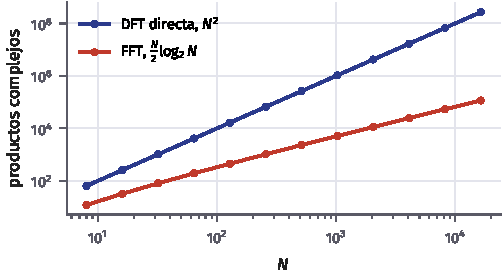
\includegraphics[width=\linewidth]{complejidad}
      \footnotesize
      \begin{center}
        \begin{tabular}{@{}rrrr@{}}
          \toprule
          $N$ & $N^2$ & $\frac N2\log_2N$ & ganancia\\\midrule
          64 & 4096 & 192 & 21\\
          1024 & $1{,}05\cdot10^6$ & 5120 & 205\\
          $2^{16}$ & $4{,}3\cdot10^9$ & $5{,}2\cdot10^5$ & 8192\\\bottomrule
        \end{tabular}
      \end{center}
    \end{column}
  \end{columns}
\end{frame}

\begin{frame}{Diezmado en el tiempo (base 2)}
  Sea $N=2^p$. Separamos las muestras pares ($n=2r$) y las impares ($n=2r+1$), y usamos $W_N^2=W_{N/2}$:
  \[
    X[k]=\sum_{r=0}^{N/2-1}x[2r]\,W_N^{2rk}+\sum_{r=0}^{N/2-1}x[2r+1]\,W_N^{(2r+1)k}
    =\underbrace{\sum_{r=0}^{N/2-1}x[2r]\,W_{N/2}^{rk}}_{F[k]}+W_N^{k}\underbrace{\sum_{r=0}^{N/2-1}x[2r+1]\,W_{N/2}^{rk}}_{G[k]}
  \]
  \begin{itemize}
    \item $F[k]$ y $G[k]$ son las DFT de $N/2$ puntos de las muestras pares e impares; son periódicas de periodo $N/2$.
    \item Como $W_N^{k+N/2}=-W_N^k$, basta calcularlas para $k=0,\dots,N/2-1$:
  \end{itemize}
  \begin{importante}[Mariposa]
    \[
      X[k]=F[k]+W_N^k\,G[k],\qquad X[k+N/2]=F[k]-W_N^k\,G[k],\qquad k=0,\dots,\tfrac N2-1
    \]
  \end{importante}
\end{frame}

\begin{frame}{La mariposa y la recursión}
  \begin{columns}[c]
    \begin{column}{0.4\textwidth}
      \begin{center}
        \begin{tikzpicture}[x=1.15cm, y=1cm, font=\footnotesize]
          \node[left] (f) at (0,1.2) {$F[k]$};
          \node[left] (g) at (0,0) {$G[k]$};
          \node[right] (x1) at (3,1.2) {$X[k]$};
          \node[right] (x2) at (3,0) {$X[k+\frac N2]$};
          \fill[pdsazul] (0,1.2) circle (1.5pt) (0,0) circle (1.5pt) (3,1.2) circle (1.5pt) (3,0) circle (1.5pt);
          \draw[flecha, pdsazul] (0,1.2) -- (3,1.2);
          \draw[flecha, pdsazul] (0,1.2) -- (3,0);
          \draw[pdsazul, thick] (0,0) -- (0.9,0);
          \node[below, pdsrojo] at (0.45,0) {$W_N^k$};
          \draw[flecha, pdsazul] (0.9,0) -- (3,1.2);
          \draw[flecha, pdsazul] (0.9,0) -- (3,0);
          \node[below, pdsrojo] at (2.6,0) {$-1$};
        \end{tikzpicture}
      \end{center}
      \small Un producto complejo y dos sumas por cada par de salidas.
    \end{column}
    \begin{column}{0.58\textwidth}
      \begin{itemize}
        \item Las DFT de $N/2$ puntos se dividen igual, hasta llegar a DFT de 1 punto ($X[0]=x[0]$).
        \item $\log_2N$ etapas de $N/2$ mariposas:
        \[
          \frac N2\log_2N\ \text{productos},\qquad N\log_2N\ \text{sumas}.
        \]
        \item La entrada queda en \alert{orden de bits invertidos}: con $N=8$, el índice $1=001_2$ va a la posición $100_2=4$.
      \end{itemize}
      \footnotesize
      \begin{center}
        \begin{tabular}{@{}lcccccccc@{}}
          \toprule
          $n$ & 0&1&2&3&4&5&6&7\\
          binario & 000&001&010&011&100&101&110&111\\
          invertido & 000&100&010&110&001&101&011&111\\
          posición & 0&4&2&6&1&5&3&7\\\bottomrule
        \end{tabular}
      \end{center}
    \end{column}
  \end{columns}
\end{frame}

\begin{frame}{FFT de 8 puntos}
  \begin{center}
    \begin{tikzpicture}[x=2.3cm, y=0.52cm, font=\scriptsize]
      \def\orden{{0,4,2,6,1,5,3,7}}
      \foreach \i in {0,...,7} {
        \pgfmathtruncatemacro{\n}{\orden[\i]}
        \node[left] at (0,-\i) {$x[\n]$};
        \node[right] at (3,-\i) {$X[\i]$};
        \foreach \c in {0,1,2,3} \fill[pdsazul] (\c,-\i) circle (1.2pt);
      }
      % etapa 1: mariposas entre vecinos
      \foreach \b in {0,2,4,6} {
        \pgfmathtruncatemacro{\a}{\b+1}
        \draw[pdsazul!70] (0,-\b) -- (1,-\b) (0,-\b) -- (1,-\a) (0,-\a) -- (1,-\b) (0,-\a) -- (1,-\a);
      }
      % etapa 2: distancia 2
      \foreach \g in {0,4} \foreach \j in {0,1} {
        \pgfmathtruncatemacro{\p}{\g+\j}
        \pgfmathtruncatemacro{\q}{\g+\j+2}
        \draw[pdsverde!80] (1,-\p) -- (2,-\p) (1,-\p) -- (2,-\q) (1,-\q) -- (2,-\p) (1,-\q) -- (2,-\q);
      }
      % etapa 3: distancia 4
      \foreach \j in {0,...,3} {
        \pgfmathtruncatemacro{\q}{\j+4}
        \draw[pdsrojo!80] (2,-\j) -- (3,-\j) (2,-\j) -- (3,-\q) (2,-\q) -- (3,-\j) (2,-\q) -- (3,-\q);
      }
      \node[pdsgris] at (0.5,1) {DFT de 2};
      \node[pdsgris] at (1.5,1) {DFT de 4};
      \node[pdsgris] at (2.5,1) {DFT de 8};
      \foreach \j in {0,...,3} \node[pdsrojo, font=\tiny, above left] at (2,-\j-4) {$W_8^{\j}$};
      \foreach \j in {0,1} \node[pdsverde, font=\tiny, above left] at (1,-\j-2) {$W_4^{\j}$};
    \end{tikzpicture}
  \end{center}
  \nota{Tres etapas de cuatro mariposas. En cada mariposa, la rama inferior se multiplica por $W_m^{k}$ y la salida inferior lleva un signo menos.}
\end{frame}

\begin{frame}{Variantes y la FFT en la práctica}
  \begin{itemize}
    \item \alert{Diezmado en frecuencia}: se separan $X[k]$ pares e impares; la salida queda en bits invertidos.
    \item Otras bases (4, 8, mixtas) y algoritmos para \alert{cualquier} $N$ (Bluestein, Rader). Las bibliotecas (FFTW, la de NumPy y la de Matlab) eligen el método según $N$; con $N$ potencia de 2 o con factores pequeños es más rápida.
    \item La \alert{IFFT} es una FFT con el signo cambiado:
    \[
      x[n]=\frac1N\Big(\sum_kX^*[k]W_N^{kn}\Big)^*=\frac1N\,\big(\operatorname{FFT}\{X^*\}\big)^*
    \]
    \item Con señales reales se aprovecha la simetría (\texttt{rfft}): la mitad de trabajo.
    \item Se puede calcular \emph{en el sitio} (sin memoria adicional) y en coma fija; es la operación estrella de los DSP.
  \end{itemize}
\end{frame}

\begin{frame}{En código: FFT en base 2}
  \codigo[basicstyle=\ttfamily\fontsize{6.8}{7.8}\selectfont]{fft_radix2}
  \nota{Cada etapa combina bloques de $m/2$ en bloques de $m$ con mariposas, tras reordenar la entrada por inversión de bits.}
\end{frame}

% =====================================================================
\section{Convolución rápida}

\begin{frame}{Convolución con la FFT}
  \begin{center}
    \begin{tikzpicture}[node distance=0.7cm, font=\small]
      \node (x) {$x[n]$};
      \node[bloque, right=of x] (fx) {FFT de\\$N$ puntos};
      \node (h) [below=0.6cm of x] {$h[n]$};
      \node[bloque, right=of h] (fh) {FFT de\\$N$ puntos};
      \node[draw, circle, inner sep=1pt, right=1.6cm of fx, yshift=-0.75cm] (p) {$\times$};
      \node[bloque, right=of p] (ifft) {IFFT};
      \node[right=of ifft] (y) {$y[n]$};
      \draw[flecha] (x) -- (fx); \draw[flecha] (h) -- (fh);
      \draw[flecha] (fx) -| (p); \draw[flecha] (fh) -| (p);
      \draw[flecha] (p) -- (ifft); \draw[flecha] (ifft) -- (y);
    \end{tikzpicture}
  \end{center}
  \begin{itemize}
    \item Con $N\ge L+M-1$ (rellenando con ceros) se obtiene la convolución \alert{lineal} (parte~2).
    \item Coste: tres FFT y $N$ productos, unos $\frac32N\log_2N+N$, frente a $LM$ de la suma directa.
    \item Con $L=M=1000$: $10^6$ productos directos frente a unos $3{,}6\cdot10^4$ con $N=2048$.
    \item Para filtros cortos ($M\lesssim50$) la suma directa sigue siendo competitiva.
    \item $H[k]$ se calcula una sola vez si se filtran muchas señales con el mismo $h$.
  \end{itemize}
\end{frame}

\begin{frame}{Señales largas: solapamiento y suma}
  \begin{columns}[c]
    \begin{column}{0.52\textwidth}
      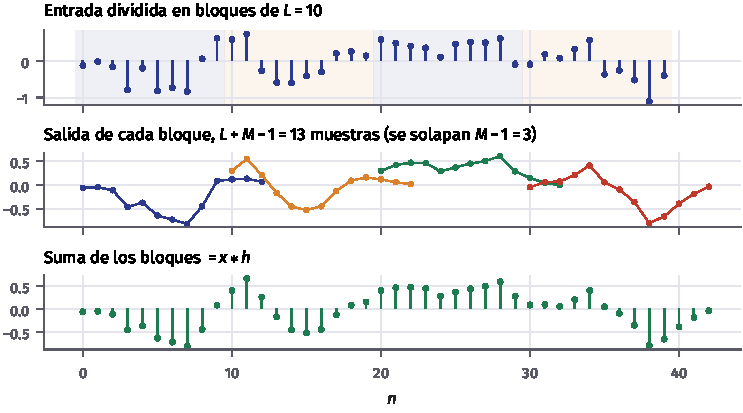
\includegraphics[width=\linewidth]{solapamiento_suma}
    \end{column}
    \begin{column}{0.46\textwidth}
      \small
      Si $x[n]$ es muy larga (o no termina), se divide en bloques de $L$ muestras, $x[n]=\sum_ix_i[n-iL]$:
      \begin{itemize}\small
        \item Cada bloque se convoluciona con $h$ por FFT de $N\ge L+M-1$ puntos.
        \item Las salidas, de $L+M-1$ muestras, se \alert{solapan $M-1$} y se suman:
        \[
          y[n]=\sum_i y_i[n-iL],\quad y_i=x_i\conv h
        \]
        \item Retardo de un bloque: apto para tiempo real.
      \end{itemize}
    \end{column}
  \end{columns}
\end{frame}

\begin{frame}{Señales largas: solapamiento y almacenamiento}
  \begin{itemize}
    \item Bloques de entrada de $N$ muestras que se \alert{solapan $M-1$} con el anterior.
    \item Se calcula la convolución \alert{circular} de $N$ puntos de cada bloque con $h$.
    \item Las $M-1$ primeras muestras están contaminadas por el plegado circular: se \alert{descartan}. Las $N-M+1$ restantes coinciden con la convolución lineal y se \alert{guardan}.
  \end{itemize}
  \begin{center}
    \footnotesize
    \renewcommand{\arraystretch}{1.2}
    \begin{tabular}{@{}lll@{}}
      \toprule
      & Solapamiento y suma & Solapamiento y almacenamiento\\\midrule
      Bloques de entrada & $L$ muestras, sin solape, + ceros & $N$ muestras, solape $M-1$\\
      Convolución & lineal (por relleno) & circular\\
      Salida & se suman los solapes & se descartan $M-1$ muestras\\\bottomrule
    \end{tabular}
  \end{center}
  \nota{Las dos dan el mismo resultado con el mismo coste. \texttt{scipy.signal.oaconvolve} y \texttt{fftfilt} de Matlab las implementan.}
\end{frame}

\begin{frame}{En código: solapamiento y suma}
  \codigo[basicstyle=\ttfamily\fontsize{6.8}{7.8}\selectfont]{solapamiento_suma}
  \nota{Bloques de 226 muestras y FFT de $N=256$: el resultado coincide con la convolución directa.}
\end{frame}

\begin{frame}{¿Y si el sistema es IIR?}
  \begin{columns}[c]
    \begin{column}{0.5\textwidth}
      \small
      Si $h[n]$ es infinita, la IDFT de $N$ muestras de $H(\e^{j\Omega})$ es su \alert{extensión periódica}:
      \[
        h_N[n]=\sum_rh[n-rN]
      \]
      \begin{ejemplo}[$h{[n]}=a^nu{[n]}$, $\abs a<1$]
        \footnotesize
        $H[k]=\dfrac{1}{1-aW_N^k}$ y $h_N[n]=\dfrac{a^n}{1-a^N}$, $0\le n<N$.
      \end{ejemplo}
      \begin{itemize}\small
        \item Con $N$ grande ($a^N\approx0$) el error es despreciable: la DFT filtra \alert{aproximadamente} con un IIR.
        \item Lo exacto (y más barato) es la ecuación en diferencias (Tema~4).
      \end{itemize}
    \end{column}
    \begin{column}{0.48\textwidth}
      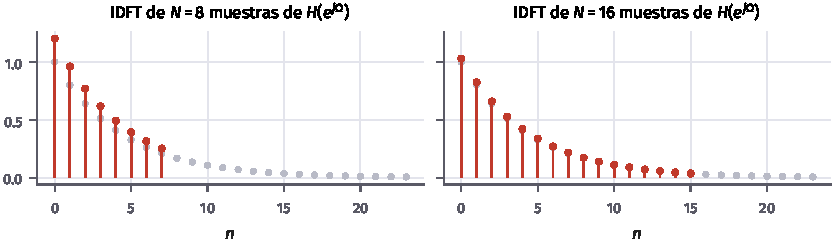
\includegraphics[width=\linewidth]{muestreo_frecuencia}
      \nota{$a=0{,}8$: con $N=8$, $h_N[0]=1/(1-0{,}8^8)=1{,}20$; con $N=16$, $1{,}03$.}
    \end{column}
  \end{columns}
\end{frame}

% =====================================================================
\section*{Resumen}
\begin{frame}{Conceptos importantes}
  \begin{columns}[T]
    \begin{column}{0.5\textwidth}
      \begin{itemize}
        \item FFT: misma DFT en $\frac N2\log_2N$ productos.
        \item Diezmado en el tiempo: $X[k]=F[k]+W_N^kG[k]$, $X[k+\frac N2]=F[k]-W_N^kG[k]$.
        \item $\log_2N$ etapas de mariposas; entrada en bits invertidos.
        \item IFFT con la misma FFT.
      \end{itemize}
    \end{column}
    \begin{column}{0.5\textwidth}
      \begin{itemize}
        \item Convolución rápida: FFT, producto, IFFT con $N\ge L+M-1$.
        \item Señales largas: solapamiento y suma o solapamiento y almacenamiento.
        \item Con IIR, la DFT da $h$ periodizada: aproximación válida si $N$ es grande.
      \end{itemize}
    \end{column}
  \end{columns}
  \bigskip
  \gris{Apuntes del Tema 3, sección 5 · Hoja de ejercicios, ejercicios 14–16.}
\end{frame}

\end{document}
